% 2013_anhui_science_q19_fig1: schematic cone with base circle seen as ellipse
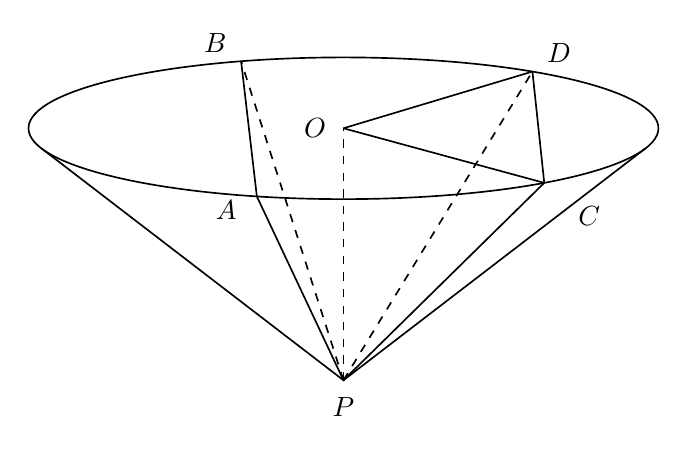
\begin{tikzpicture}[x=1cm,y=1cm,font=\normalsize,line width=.6pt]
\coordinate (P) at (0,-1.2);
\coordinate (O) at (0,2.0);
\coordinate (B) at (-1.3000000000,2.8511426144);
\coordinate (A) at (-1.1000000000,1.1347001965);
\coordinate (D) at (2.4000000000,2.7200000000);
\coordinate (C) at (2.5500000000,1.3065946802);
% base ellipse
\draw[solid] (0,2.0) ellipse (4.0 and 0.9);
% generators and verticals
\draw[solid] (P) -- (A);
\draw[solid] (P) -- (C);
\draw[solid] (B) -- (A);
\draw[solid] (D) -- (C);
\draw[solid] (O) -- (D);
\draw[solid] (O) -- (C);
\draw (-3.8385381332,1.7468750000)--(P)--(3.8385381332,1.7468750000);
% hidden
\draw[dashed] (P) -- (B);
\draw[dashed] (P) -- (D);
\draw[dashed] (P) -- (O);

% labels with clearance
\node[inner sep=2pt,below=4pt] at (P) {$P$};
\node[inner sep=2pt,left=4pt] at (O) {$O$};
\node[inner sep=2pt,above left=4pt,xshift=1pt,yshift=-3pt] at (B) {$B$};
\node[inner sep=2pt,left=4pt,xshift=-1pt,yshift=-5pt] at (A) {$A$};
\node[inner sep=2pt,above right=4pt,xshift=-1pt,yshift=-3pt] at (D) {$D$};
\node[inner sep=2pt,right=4pt,xshift=6pt,yshift=-12pt] at (C) {$C$};
\end{tikzpicture}
